\documentclass{beamer}
\usepackage[utf8]{inputenc}
\usepackage{amsfonts,url}
\usepackage{verbatim}
\usepackage{tikz}
\usetikzlibrary{ automata, positioning, arrows}



\usetheme{Goettingen}
\usecolortheme{beaver}


\newcommand{\NN}{\mathbb{N}}
\newcommand{\ZZ}{\mathbb{Z}}
\newcommand{\wi}{\mathbf{w}}
\newcommand{\vi}{\mathbf{v}}
\newcommand{\ui}{\mathbf{u}}
\newcommand{\QQ}{\mathcal{Q}}
\newcommand{\FF}{\mathcal{F}}
\newcommand{\auto}{\mathcal{A}}


\title{Groups of  Automata}
\author{Carlo Lanzi Luciani}
\institute{Mentor: prof. Ganna Kudryavtseva}
\date{\today}

\begin{document}
%1title frame
\begin{frame}
  \titlepage{}
\end{frame}

%2intention's declaration
\begin{frame}
\frametitle{1.Introduction}
 Automata are found to be important in:
\begin{itemize}
\item Information Theory
\item Theory of Dynamical System
\item Algebra
\item Other areas
\end{itemize}
\begin{block}{My Aim}
Study some of the groups constructed through a special class of them, the Mealy Automata
%here i can mention Grigorchuk group and the burnside problem
% so the intermediate growth, between polynomial and exponential, and the concept of growth of a group
\end{block}
\end{frame}


%2superbrief intro on word spaces
\begin{frame}
\frametitle{2.Alphabet and the Free Monoid}
Let $X$ be finite set, called the \textit{Alphabet}. Then we have:\begin{itemize}
\item $X^*=\{x^{1}x^{2}\ldots x^{n}:x^{i}\in X, n\in\NN\}$ the \textit{Free Monoid}
\item Composition of words: $\wi\circ\vi:=\wi \vi$
\item The Empty Word $\varnothing$
\item Lenght of words: $\wi=x_1 \ldots x_n , |\wi|:=n$
\end{itemize}
\end{frame}




\begin{comment}
\item Alphabet Tree:
\begin{figure}[ht]
\centering
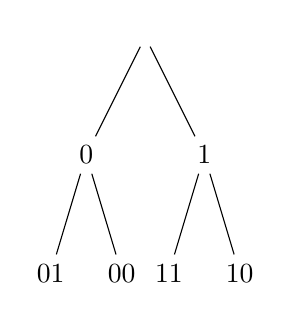
\begin{tikzpicture}

\node {$\varnothing$}
    child {  node {$0$}  child[right] { node {$01$} }
                    child[left] { node {$00$} } }
    child {  node {$1$}
                    child[right] { node {$11$} }
                    child[left] { node {$10$} }
             }  ;
\end{tikzpicture}
\caption{An example in the case $X=\{0,1\}$}
\end{figure}
\end{comment}




%picture of an  Automata
\begin{frame}
\frametitle{3.An Example with Moore Diagrams}
\begin{block}{Moore Diagrams}
We put $G=(\QQ,E)$ with $E:=\{(q_i,q_j)|\exists \wi \in X : \pi(\wi,q_i)=q_j\}$
\end{block}
\begin{figure}[ht]
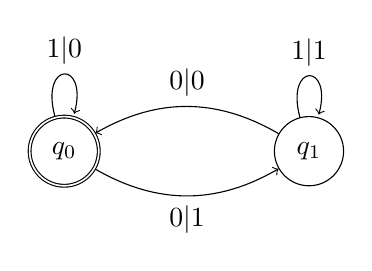
\begin{tikzpicture}
\node[state, accepting](q0) at (0,0) {$q_0$};
\node[state, right of=q0, xshift=60] (q1) {$q_1$};
\draw	(q0) edge[below,bend right,->] node{$0|1$} (q1)
		(q0) edge[loop above] node{$1|0$} (q0)
		(q1) edge[loop above] node{$1|1$} (q1)
		(q1) edge[above, bend right,->] node{$0|0$} (q0);
		
\end{tikzpicture}
\caption{Example of a Moore Diagram of a 2-state Synchonous Automaton over the alphabet $X_I=X_O=X=\{0,1\}$}
\end{figure}
 
%Here instead of giving the exact definition of the extension I explain it through the graph
\end{frame}




%introduction to Automata
\begin{frame}
\frametitle{4.Synchronous Automaton}
\begin{Definition}
A \textbf{Finite Synchronous  Automaton} is a set $\auto=<X_I,X_O,\QQ,\pi,\lambda>$ where:
\begin{itemize}
	\item $X_I$ and $ X_O $ are \textit{finite} sets called respectively the \textit{\textbf{Input \emph{and} Output Alphabets}}
	% so here we declare what we put inside and what comes aoutside of the machine
	\item $\QQ$ is a \emph{finite} set called the \textit{\textbf{Set of Internal States of the  Automaton}}
	\item $\pi:X_I\times\QQ \longrightarrow \QQ $ is a function called the \textit{\textbf{Transition Function}}
	\item $\lambda:X_I\times\QQ \longrightarrow X_O $ is a function called the \textit{\textbf{Output Function}}
\end{itemize}
\end{Definition}
%Here I give the concept through the graph and I invite the people to observe intuitively the concept
\end{frame}




\begin{frame}
\frametitle{5.Extension of $\pi$ and $\lambda$}
\begin{block}{Observation}
We can naturally extend the Domain of $\pi$ and $\lambda$:
\begin{itemize}
	\item $\pi:X_{I}^{*} \times \QQ:\longrightarrow \QQ $
	$$\pi(\varnothing,q)=q$$ $$\pi(\wi x,q)=\pi(\wi,\pi(x,q))$$
	\item $\lambda:X_{I}^{*} \times \QQ:\longrightarrow X_{O}^{*}$
	$$\lambda(\varnothing,q)=\varnothing$$ $$\lambda(\wi x,q)=\lambda(\wi,\pi(x,q))\lambda(x,q)$$
\end{itemize}
\end{block}
\end{frame}






\begin{frame}
\frametitle{6.Action of an  Automaton}
\begin{Definition}
If an  Automaton $\auto$ has a fixed state $q_0$ we call it an \textit{Initial  Automaton} and we write it as $\auto_{q_0}$
\end{Definition}

\begin{block}{Observation}
Each $\auto_{q_0}$ naturally defines $f:{X_I}^*\longrightarrow {X_O}^*$, with $f(\wi):=\lambda(\wi,q_0)$, called \emph{Action of the  Automaton $\auto_{q_0}$}
%Here I draw on the board giving the concept a machine that simply takes some text and gives out some other
\end{block}
\end{frame}





\begin{frame}
\frametitle{7.Composition of  Automata}
\begin{Definition}
Given $\auto_1=<X_I,X_{IO},\QQ_1,\pi_1,\lambda_1>$ and $\auto_2=<X_{IO},X_O,\QQ_2,\pi_2,\lambda_2>$ we define their \emph{composition} $\mathcal{B}=\auto_1*\auto_2=<X_I,X_O,\QQ_1\times\QQ_2,\pi,\lambda>$ with $\pi$ and $\lambda$ as follows:
\begin{itemize}
\item $\pi(x,(s_1,s_2))=(\pi_1(x,s_1),\pi_2(\lambda_1(x,s_1),s_2))$
\item $\lambda(x,(s_1,s_2))=\lambda_2(\lambda_1(x,s_1),s_2)$
\end{itemize}
\textbf{Observe:}
(Action of $\auto_2$)$\circ$(Action of $\auto_1$)=Action of $\auto_1*\auto_2$
% Here I take again the same concept and I link 2 machines 1 after the other
\end{Definition}
\end{frame}



\begin{frame}
\frametitle{8.Some Algebraic Results}
\begin{block}{Consequences}
From now on we assume that $X=X_I=X_O$:
\begin{itemize}

\item The functions $f:X^*\longrightarrow X^*$ defined by Mealy  Automata(called \textbf{synchronous automatic}) form a \emph{semigroup}
\item Let $\auto$ be a Synchronous  Automaton with its action $f$. It's invertible \textbf{(exists $\auto'$ with its action $f'$ such that $f\circ f'=id$)} \emph{if and only if} $\lambda(\cdot,q) $ is invertible 

(Memento: $\lambda(\cdot ,q) $ is exactly the action of the  Automaton)
$$x|y\longrightarrow y|x$$
\end{itemize}
\end{block}

\end{frame}




\begin{comment}
\begin{Definition}
$\auto$ is a \textbf{Mealy  Automaton} (also called \textbf{Sinchronous  Automaton}) if $\forall x\in X$, we have $|\lambda_q(x)|=|\lambda(x,q)|=1$
\end{Definition}
[\textbf{Note:} Asynchronus $\neq$ Synchronous]
\begin{Definition}
\item The functions $f: X^* \longrightarrow X^*$ defined by Asynchronous  Automata form a \emph{semigroup}
\item $f$ is Synchronous Automatic \emph{if and only if} is a \textbf{Tree Homomorphism} on $X^*$, i. e. 
\begin{itemize}
\item $f(root)=root$ 
\item if $(\wi,\vi)$ is an edge $\Rightarrow  (f(\wi),f(\vi)) $ is an edge in the image tree
\end{itemize}
\end{comment}




\begin{frame}
\frametitle{9.Groups of Synchronous  Automata}
\begin{Definition}
Let $\auto$ be a Synchronous Invertible  Automata. The \textit{Group Defined by the Invertible  Automaton $\auto$} is the group generated by the actions defined by $\{\auto_q:q\in\QQ\}$
\end{Definition}
\begin{block}{Proposition}
Let $\auto$ be a 2-state  Automaton over the alphabet $X=\{0,1\}$ and $G$ the group defined by this  Automaton. Then $G$ is isomorphic to one of the following group:
\begin{itemize}
\item \textit{the trivial group} $\{1_G\}$
\item $\ZZ_2$
\item $\ZZ_2\oplus\ZZ_2$
\item $\ZZ$
\item \textit{the Infinite Dihedral group} $\mathbb{D}_\infty$
\item \textit{the Lamplighter group} $\ZZ\wr\ZZ_2$
\end{itemize}
\end{block}
\end{frame}


%I don't know if it's the right thing to do to give grigourchoup group, otherwise i'll have to explain everything through slides




\begin{frame}
\frametitle{10.Conclusion}
\begin{figure}[ht]
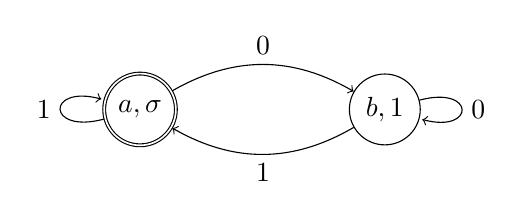
\begin{tikzpicture}
\node[state, accepting] (a) at (0,0) {$a,\sigma$};
\node[state, right of=a, xshift=60] (b) {$b, 1$};
\draw	(a) edge[left, loop left, ->] node{$1$} (a)
		(a) edge[bend left,->, above] node{$0$} (b)
		(b) edge[loop right, ->, right] node{$0$} (b)
		(b) edge[below, bend left,->] node{$1$} (a);
		
\end{tikzpicture}
\caption{Automaton which defines the Lamplighter group}
\end{figure}
\begin{block}{Actual Progress}
At present, in the case of a \textit{3-state Automaton} over a \textit{2-letter Alphabet} are classified just the finite, abelian and free groups 
\end{block}
\end{frame}






\begin{frame}
\begin{huge}
Thank you for your attention!
\end{huge}
\end{frame}

\begin{comment}
\begin{frame}
\frametitle{The Lamplighter Group*}
\begin{block}{Ingredients}
\begin{itemize}
\item Direct sum of $\ZZ_2$ on $\ZZ$:
$${\ZZ_2}^{(\ZZ)}=\bigoplus_{j\in\ZZ} {\ZZ_2}^{j}:=\{(b_j)_{j\in \ZZ}| b \in \ZZ^2, b_j\neq 0\textrm{ for a finite number of j}\}$$
\item Action through Translation of $\ZZ$ on $\ZZ_2$:
$$\phi:\ZZ\times{\ZZ_2}^{(\ZZ)}\longrightarrow\ZZ_2$$ $$\phi(z,(b_j)_{j\in\ZZ}):=(b_j)_{j-z\in\ZZ}$$
\end{itemize}
\end{block}
\begin{block}{Definition of $\ZZ\wr\ZZ_2$}
The Lamplighter group is the set $\ZZ\times{\ZZ_2}^{(\ZZ)}$ provided with the operation:
$$(z_1,({b^1}_j)_{j\in\ZZ})*(z_2,({b^2}_j)_{j\in\ZZ}):=(z_1 +z_2,({b^1}_j+{b^2}_{j-z_1})_{j\in\ZZ})$$
\end{block}
\end{frame}
\end{comment}

\end{document}